\documentclass{ctexart}
\usepackage{array}
\usepackage{amsmath}
\usepackage{amssymb}
\usepackage{enumerate}
\usepackage{amsthm}
\usepackage{bm}
\usepackage{mathtools}
\usepackage{mathrsfs}

\usepackage{indentfirst}
\usepackage{setspace}
\usepackage{subfigure} 

\usepackage{tkz-fct}
\usetikzlibrary{calc,intersections,through,backgrounds,3d}
\usepackage{tkz-euclide}
\usepackage{pgfplots}

\usepackage{float}
\usepackage{graphics}
\usepackage[graphicx]{realboxes}
%\usepackage{mathpazo}
\usepackage[libertinus]{newtx}
\usepackage{fancyhdr}

\renewenvironment{proof}[1][证明]{\par\underline{\textbf{#1.}} \;\fangsong}{\qed\par}
\newenvironment{solution}{\par\underline{\textbf{解.}} \;\fangsong}{\qed\par}

\linespread{2}
\usepackage{geometry}
\geometry{a4paper,left=0.5in,right=0.5in,top=1in,bottom=1in}
\usepackage[hidelinks,colorlinks,linkcolor=blue]{hyperref}
\usepackage{color}
\newcommand{\oneb}{\underline{\hspace{1em}}\hspace{0.001em}}
\newcommand{\twob}{\oneb\oneb}
\newcommand{\fourb}{\twob\twob}
\newcommand{\tenb}{\twob\twob\twob\twob\twob}
\newcommand{\tideparallel}{%  
	\mathrel{%  
		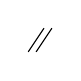
\begin{tikzpicture}[scale=0.2, baseline={([yshift=-0.5ex]current bounding box.center)}]  
			\draw[thin] (0,0) -- (1,1.5);  
			\draw[thin] (0.5,0) -- (1.5,1.5);  
		\end{tikzpicture}%  
	}%  
}  
	\newcommand{\fourch}[4]
	{\\[3pt]
		\begin{tabular}
			{*{4}{@{}p{5cm}}}
			A.~#1 & B.~#2 & C.~#3 & D.~#4
		\end{tabular}	
	}
	\newcommand{\fourchh}[4]
	{\\[5pt]
		\begin{tabular}
			{*{4}{@{}p{20cm}}}
			A.~#1 \\[5pt] B.~#2 \\[5pt] C.~#3 \\[5pt] D.~#4
		\end{tabular}	
	}
	\newcommand{\fourchhh}[4]
	{\\[3pt]
		\begin{tabular}
			{*{4}{@{}p{7.5cm}}}
			A.~#1 & B.~#2 \\[2pt] C.~#3 & D.~#4
		\end{tabular}	
	}
\everymath{\displaystyle}



\begin{document}

\pagestyle{fancy}
\lhead{}
\chead{illusion}
\rhead{\today}


\begin{enumerate}[1.]
	
\item 设 \( A \in \mathbb{F}^{m \times n} \). 那么由 Guass-Jordan 消元法知道 \( A \) 可以通过初等行变换变为行阶梯型矩阵,即满足下面两个条件:
\begin{enumerate}[(i)]
	\item 如果第 \( r \ (1 \leq r \leq m-1) \) 行元全为零,那么第 \( r+1 \) 行元也全为零.
	\item 如果第 \( l+1 \ (2 \leq l \leq m) \) 行存在非零元,则该行首个非零元所在的列数,必定大于第 \( l \) 行首个非零元所在的列数.
\end{enumerate}

显然 \( A \) 的行阶梯型矩阵不唯一,因为可以作任意次数的倍法变换. 现在对行阶梯型矩阵进一步进行初等行变换,希望得到简化行阶梯型矩阵,额外满足下面两个条件:
\begin{enumerate}[(i)]
	\item 存在非零元素的行的第一个非零元为 1;
	\item 存在非零元素的行的第一个非零元所在列的其他行的元素为 0.
\end{enumerate}

问给定 \( A \) 后,简化行阶梯型矩阵是否唯一? 

\textbf{思路参考}:如果不唯一,说明 \( AX=O \) 可选取的自由未知量发生了变化,从这一点似乎可以说明存在非零元素的行的第一个非零元所在列为固定的,但还未尝试该方法。考虑到初等变换将会在第一章讲授,是否可以单纯从矩阵的角度来解决这个问题呢?

\begin{proof}
	
\end{proof}

\newpage


\item 我们知道初等变换解决线性方程组问题的核心在于初等变换前后的两个线性方程组是同解的. 换言之,在学习可逆矩阵之后,若 \( P \) 为 \( n \) 阶可逆矩阵,那么 \( PAX=O \) 和 \( AX=O \) 自然同解. 

再考虑另一个方面,我们知道简化行阶梯矩阵虽然已经很完美了,尤其是如果你只是想解一个 \( AX=O \) 或者 \( AX=\beta \),那么将 \( A \) 化为简化行阶梯矩阵后,就可以非常轻松地得到同解方程组,进而得到基础解系. 

但从第一章的目标来看,简化行阶梯矩阵并不是相抵关系下的最简代表元. 设 \( A \) 的简化行阶梯矩阵为 \( K \),且存在可逆矩阵 \( P \),使得 \( A=PK \). 那么 \( K \) 必定可以经过若干次列初等变换变为 \( A \) 的相抵标准型. 换言之,存在 \( m \) 阶可逆矩阵 \( Q \),使得 
\[ KQ=\begin{bmatrix}
	E_r & O \\
	O & O
\end{bmatrix}=: \Lambda, \; r=r(A). \]

但这给解方程带来了一些小麻烦,在上述记号下,我们事实上得到 \( P^{-1}\Lambda Q^{-1}X=O \leadsto \Lambda Q^{-1}X=O \). 这说明 \( Q^{-1}X \) 的前 \( r \) 行都为 0. 问题来了:能从 \( Q \) 矩阵中直接读取出 \( AX=O \) 的基础解系的信息吗? 

\textbf{提示}:将 \( Q \) 按列分块,\( Q=(q_1,\cdots,q_r,q_{r+1},\cdots,q_m) \),其实 \( q_{r+1},\cdots,q_m \) 就为方程组 \( AX=O \) 的基础解系,此法称为线性方程组的公式解. 

但是我更关心的是,能不能给出一种合理的动机,自然而然给出这一点,而不是直接依赖给出结论,然后证明之. 一个自然的想法,其实对 \( K \) 作列初等变换的过程就是把原先每列对应的变量 \( x_1,\cdots,x_m \) 换成了新的变量 \( y_1,\cdots,y_m \). 并且 \( y_1,\cdots,y_m \) 可以表示为 \( x_1,\cdots,x_m \) 的线性组合.

进一步,我们希望得到 \( AX=\beta \) 的公式解,那么此时势必就要用到 \( P \) 的信息了. 事实上,有如下结论. 若 \( P\beta=(b_1,\cdots,b_m)' \),那么 \( AX=\beta \) 有解的充分必要条件为 \( b_{r+1}=\cdots=b_m=0 \),且 \( \gamma=b_1q_1+\cdots+b_rq_r \) 给出了 \( AX=\beta \) 的一个特解. 



\begin{proof}
	
\end{proof}

\newpage

\item 给定数域 \( \mathbb{F} \) 上的 \( n \) 线性空间 \( V \). 考虑 \( V \) 中 \( n^2 \) 个向量组成的向量组 \( \{\alpha_{ij}\}_{1 \leq i,j \leq n} \). 对每一个 \( i \),都有 \( \{\alpha_{ij}\}_{1 \leq j \leq n} \) 为 \( V \) 的一组基. 现在考虑如下 “形式” 矩阵:
\[ \begin{bmatrix}
	\alpha_{11} & \alpha_{12} & \cdots & \cdots & \alpha_{1n} \\
	\alpha_{21} & \alpha_{22} & \cdots & \cdots & \alpha_{2n} \\
	\alpha_{31} & \alpha_{32} & \cdots & \cdots & \alpha_{3n} \\
	\vdots & \vdots & \ddots & \ddots & \vdots \\
	\alpha_{n1} & \alpha_{n2} & \cdots & \cdots & \alpha_{nn} \\
\end{bmatrix}
\]

现在问:能否对第 \( 2 \sim n \) 行都能经过合适的调换顺序,变为 \( \alpha_{i,f(i)_1},\cdots,\alpha_{i,f(i)_n} \),其中 \( \{f(i)_1,\cdots,f(i)_n\} \) 为 \( \{1,2,\cdots,n \} \) 的一个置换,使得上述 “形式” 矩阵在调换顺序后,能够保证每一列也构成 \( V \) 的一组基. 

即对任意 \( 1 \leq j \leq n \) 都有 \( \{\alpha_{1j},\alpha_{2,f(2)_j}, \alpha_{3,f(3)_j},\cdots,\alpha_{n,f(n)_j}\} \) 为 \( V \) 的一组基. 上述记号可能不太好,我先拟的,也可以换一个你喜欢的记号. 在同构意义下,考虑 \( V \) 和 \( \mathbb{F}^n \) 没什么不同,不过问题的难度没有任何改变. 不妨只考虑 \( n=3 \) 的情形,对一般的 \( n \) 这个命题似乎还只是一个未被解决的猜想. 另外还有一个和这个类似的命题如下,请你尝试一同证明.

设 \( \{\beta_1,\cdots,\beta_n \}, \; \{\gamma_1,\cdots,\gamma_n \}\) 为 \( V \) 的两组基,是否存在 \( \{1,\cdots,n\} \) 的一个排列 \( \{ i_1,\cdots,i_n\} \),使得 \( \{\beta_1,\cdots,\beta_{j-1},\gamma_{i_j},\beta_{j+1}, \\ \cdots,\beta_n\} \) 对任意 \( 1 \leq j \leq n \) 都为 \( V \) 的一组基?


\begin{proof}
	
\end{proof}

\end{enumerate}

\end{document}
